

\section{Implementation}
\label{sec:implementation}

The implementation..

\begin{enumerate}
	\item The extra things we did to make the thing actually run
	\item Code architecture
	\item Optimizations
\end{enumerate}


\begin{figure}[htbp]
	\centering
	
	% Top row: (a), (b), (f)
	\begin{subfigure}[b]{0.45\textwidth}
		\centering
		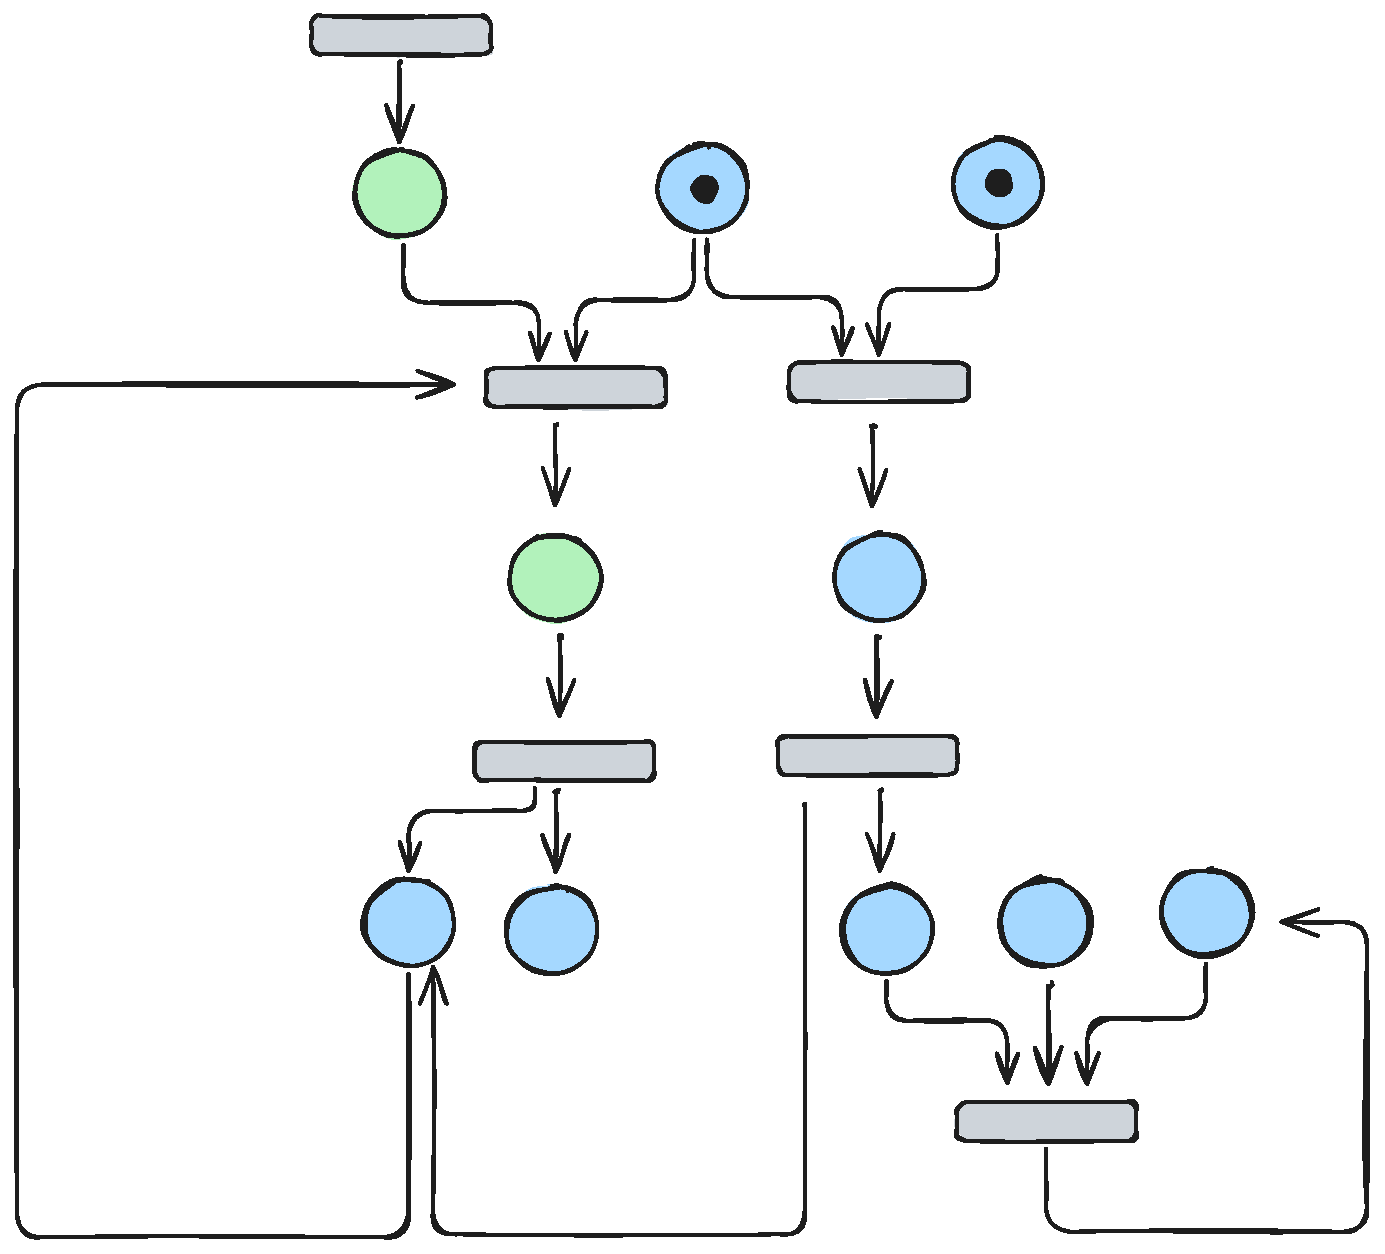
\includegraphics[width=\textwidth]{plots/bidirectional_pruning_step_a_init.pdf}
		\caption{Step 0: initial petri net, before pruning.}\label{fig:step:a}
	\end{subfigure}\hfill
	\begin{subfigure}[b]{0.45\textwidth}
		\centering
		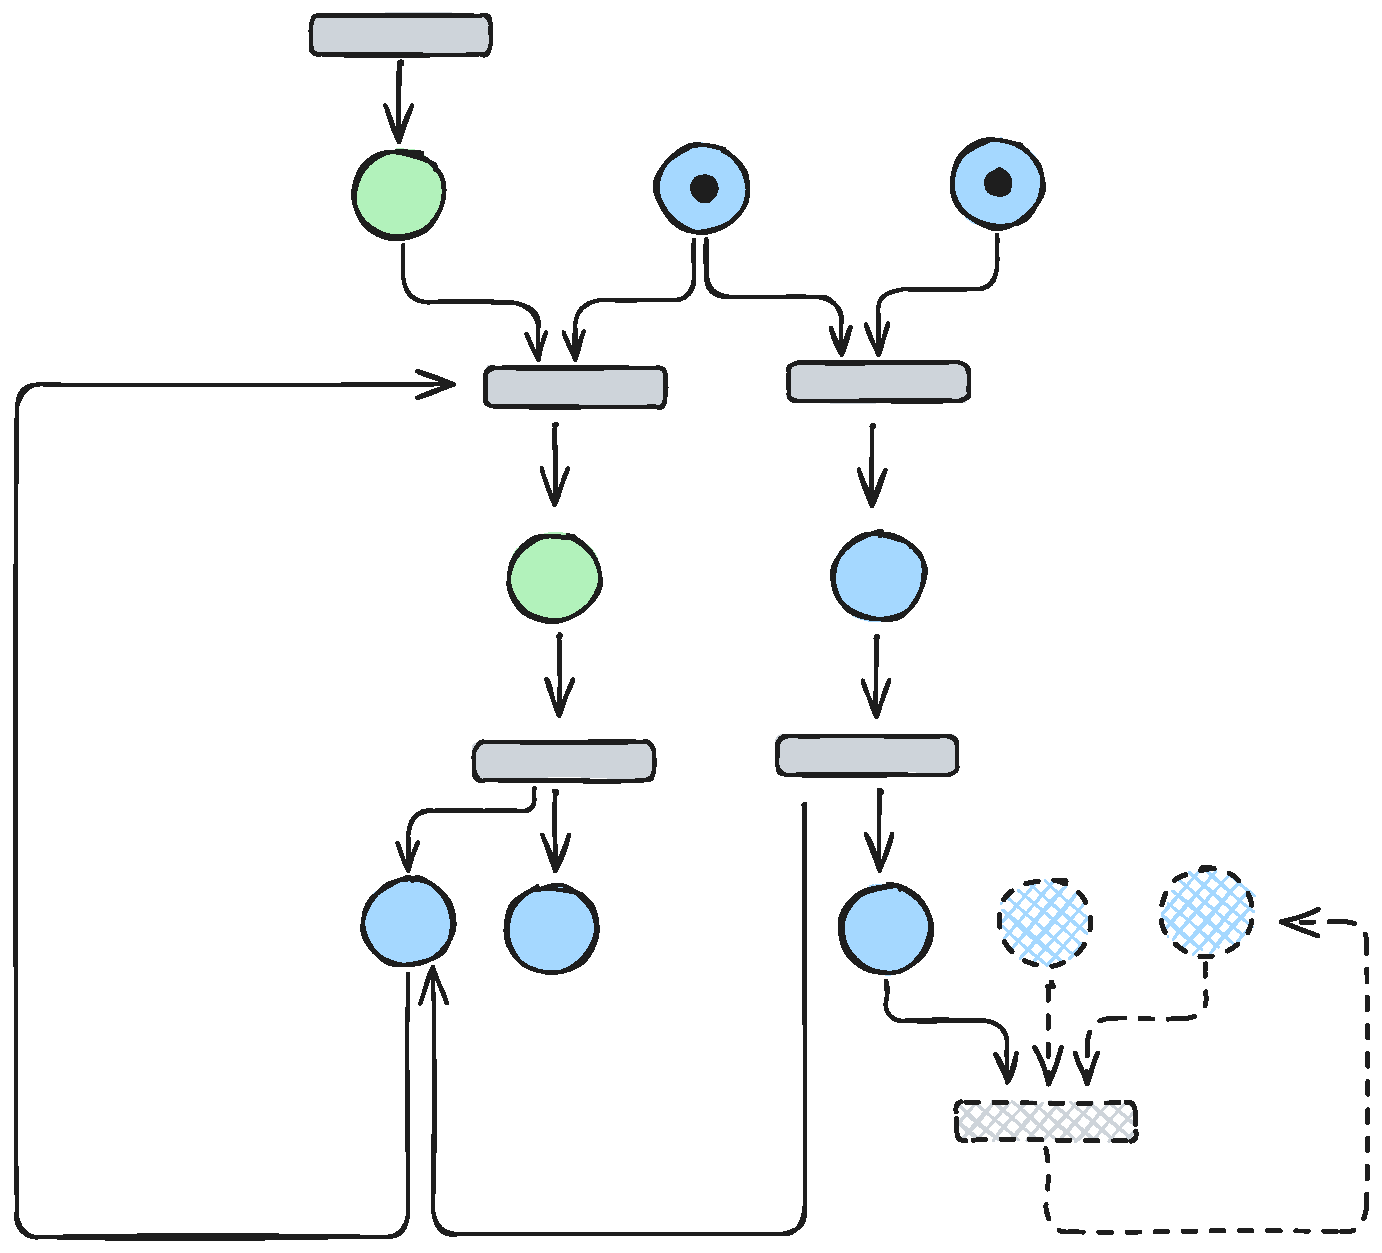
\includegraphics[width=\textwidth]{plots/bidirectional_pruning_step_b_forward.pdf}
		\caption{Step 1: during forward pass.}\label{fig:step:b}
	\end{subfigure}\hfill
	
	
	\vspace{1em}
	
	% Bottom row: (c), (d), then stacked (e)/(f) slot
	\begin{subfigure}[b]{0.30\textwidth}
		\centering
		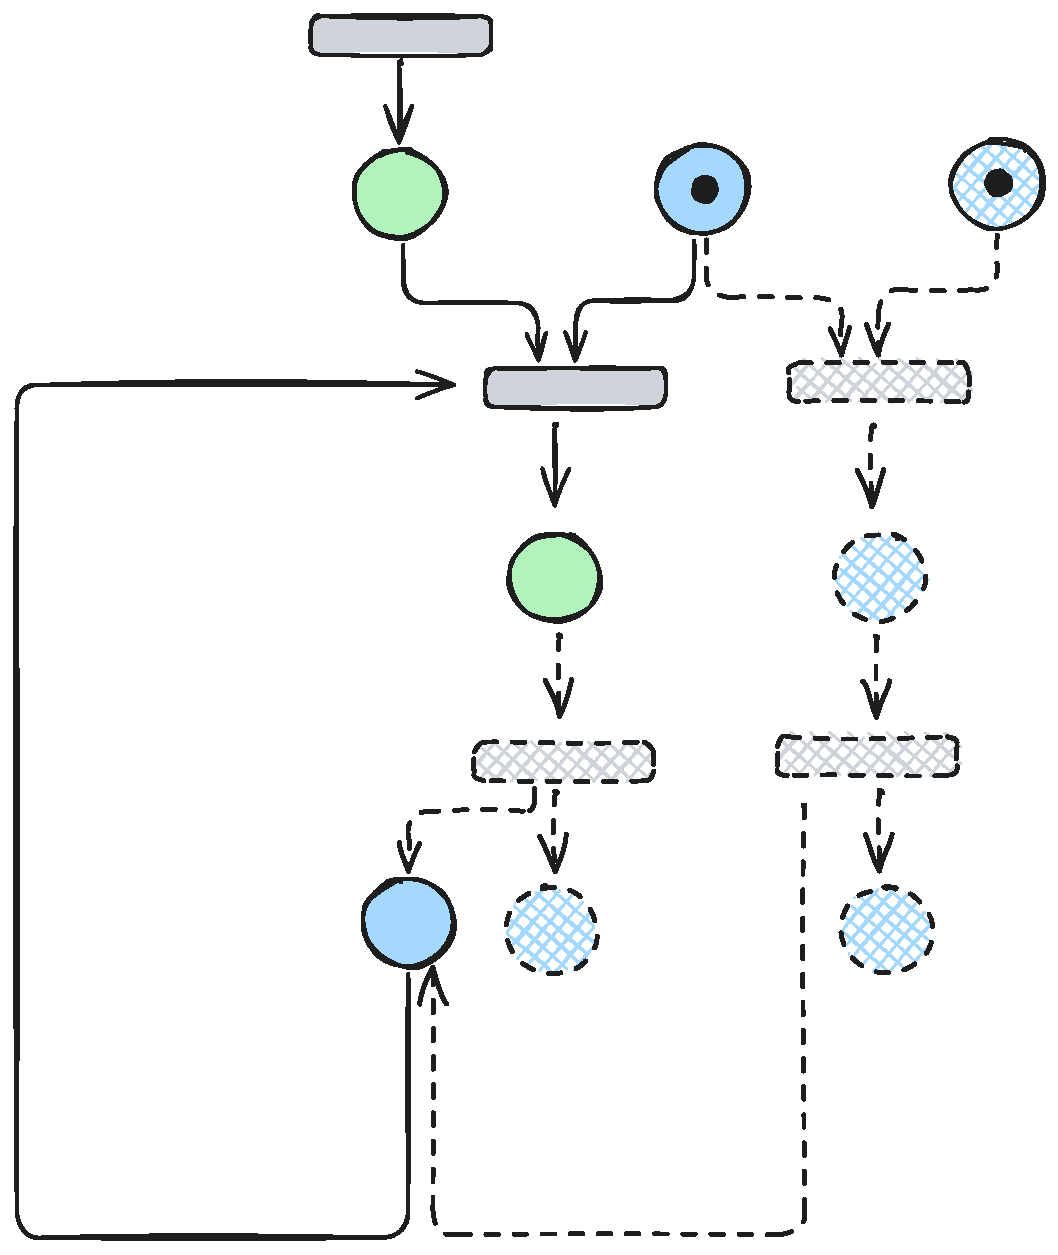
\includegraphics[width=\textwidth]{plots/bidirectional_pruning_step_c_backward.pdf}
		\caption{Step 3: after forward pass, and during backward pass.}\label{fig:step:c}
	\end{subfigure}\hfill
	\begin{subfigure}[b]{0.23\textwidth}
		\centering
		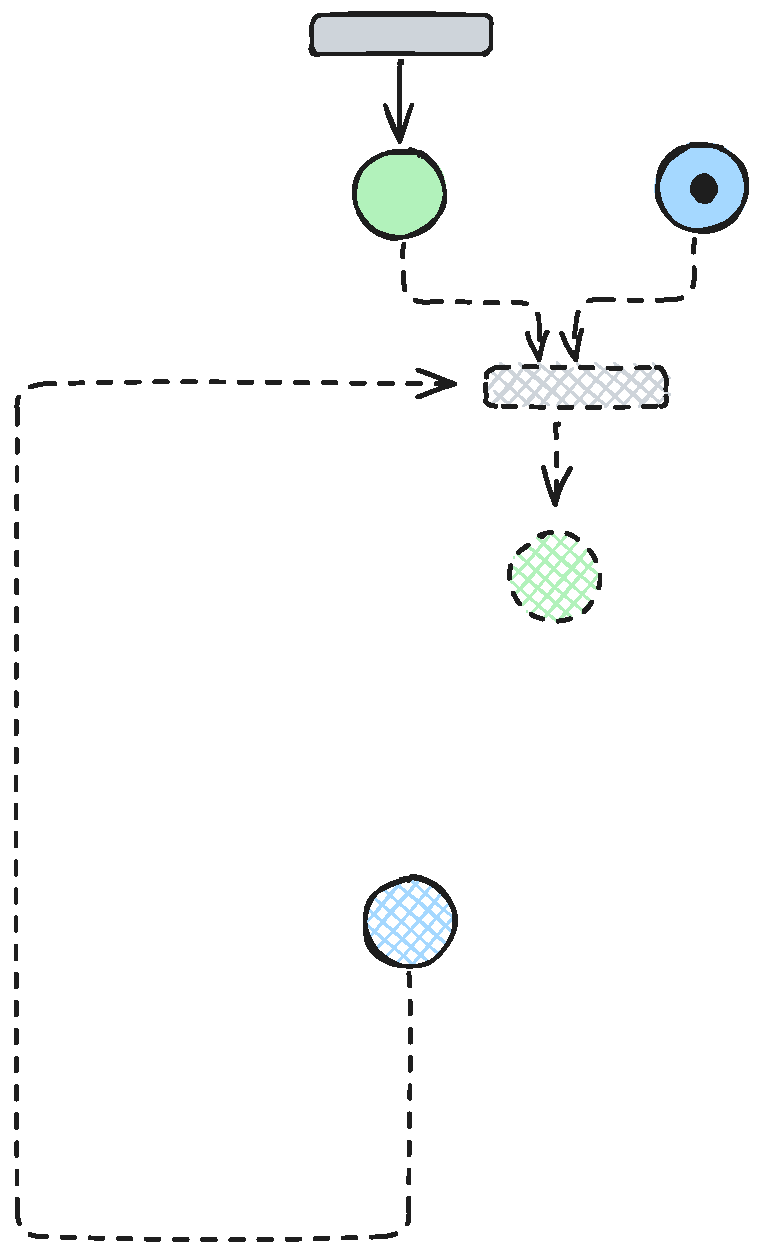
\includegraphics[width=\textwidth]{plots/bidirectional_pruning_step_d_forward.pdf}
		\caption{Step 4: after backward pass, and during forward pass.}\label{fig:step:d}
	\end{subfigure}\hfill
	\begin{subfigure}[b]{0.23\textwidth}
		\centering
		% nested for (e)
		\begin{subfigure}[b]{\textwidth}
		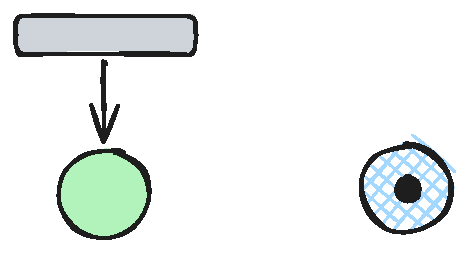
\includegraphics[width=0.5\textwidth]{plots/bidirectional_pruning_step_e_backward.pdf}
			%	       \vspace{-0.5ex}  
%			\raisebox{17ex}{%
%				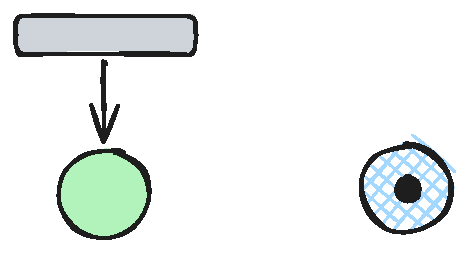
\includegraphics[width=0.65\textwidth]{plots/bidirectional_pruning_step_e_backward.pdf}%
%			}
			%		\captionsetup{skip=-15.5ex}
			\caption{Step 5: after forward pass, and during backward pass.}\label{fig:step:e}
		\end{subfigure}
		
		\vspace{0.5em}
		
		% nested for (f)
		\begin{subfigure}[b]{\textwidth}
			\centering
			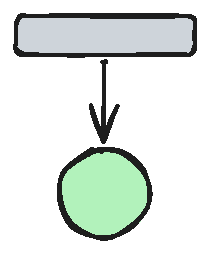
\includegraphics[width=0.23\textwidth]{plots/bidirectional_pruning_step_f_final.pdf}
			\caption{Step 6: final petri net.}\label{fig:step:f:bottom}
		\end{subfigure}
	\end{subfigure}
	
	\caption{A Petri Net after four iterations of bidirectional pruning: two forward passes and two backward passes. Black dots represent initial token markings; green places represent places that are allowed to be reachable in our constraints. Dashed shapes represent places and transitions that are identified as removable in the current iteration, and will be removed after it ends.}
	\label{fig:bidirectional_pruning}
\end{figure}




\newpage